\section{NGS}

\paragraph*{Problems with Sanger DNA sequencing}

\begin{enumerate}
	\item \textbf{Sensitivity} - Sanger technology, as well as other
technologies, do not allow to read the signal from a single DNA 
molecule. Therefore, the fragment of DNA to be sequenced 
must be amplified and the signal is obtained from many 
identical fragments. This requires \textbf{bacterial cloning}. 
A very major bottleneck.
	\item \textbf{Electrophoresis} - Sanger technology 
requires the separation of the sequencing 
reaction by individual electrophoresis, which 
is another major bottleneck of the technology.
\end{enumerate}


To prepare a NGS libraries you need to have DNA fragments and some adapters,
and you need to attach Adapters to DNA fragments (see figure \ref{fig:ngs})

\begin{figure}[H]
  \centering
  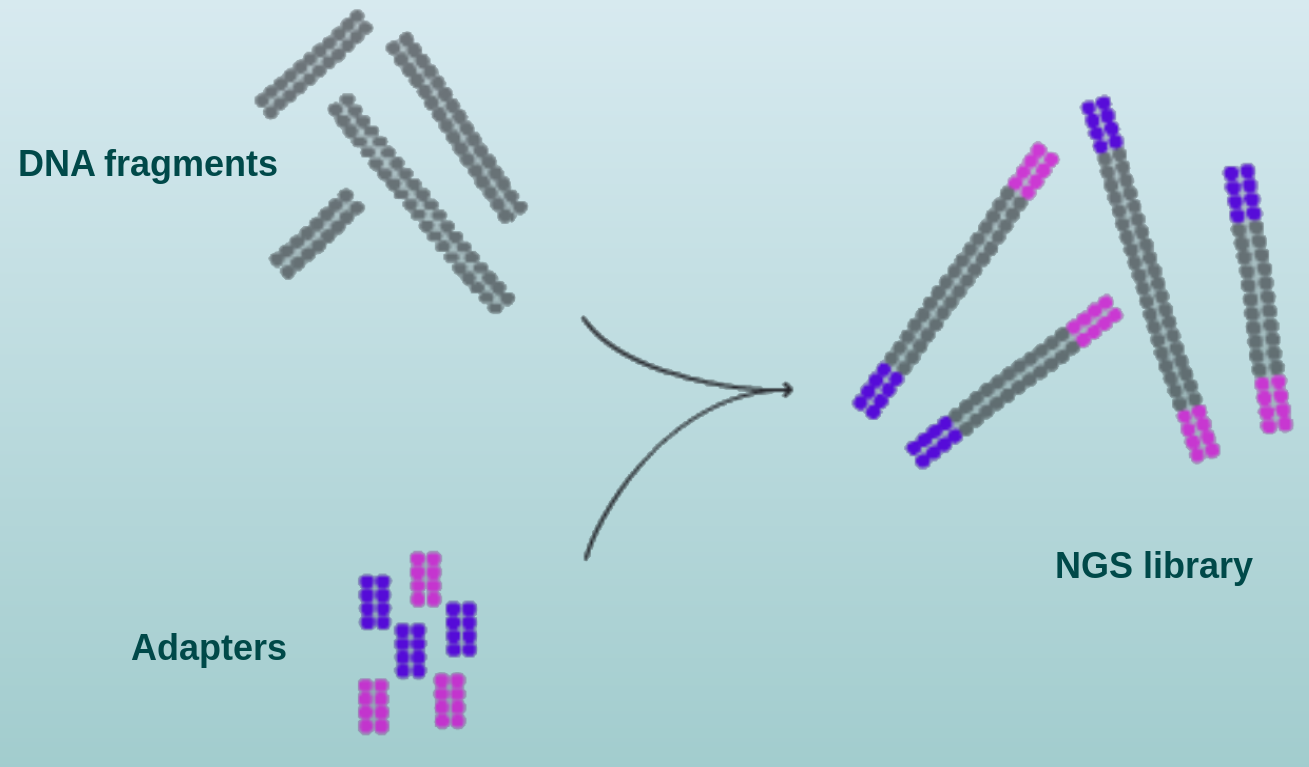
\includegraphics[scale=0.2]{ngs}
  \caption{Preparation of NGS libraries}
  \label{fig:ngs}
\end{figure}

NGS doesn't use cloning in bacteria, but use PCR - Colonies (Polonies), so DNA
is not mixed. 

\textbf{Emulsion PCR} (ePCR) is a PCR variation that some NGS technologies use to replicate DNA sequences. 
It is conducted on a bead surface within tiny water bubbles floating on an oil solution.

\begin{figure}[H]
  \centering
  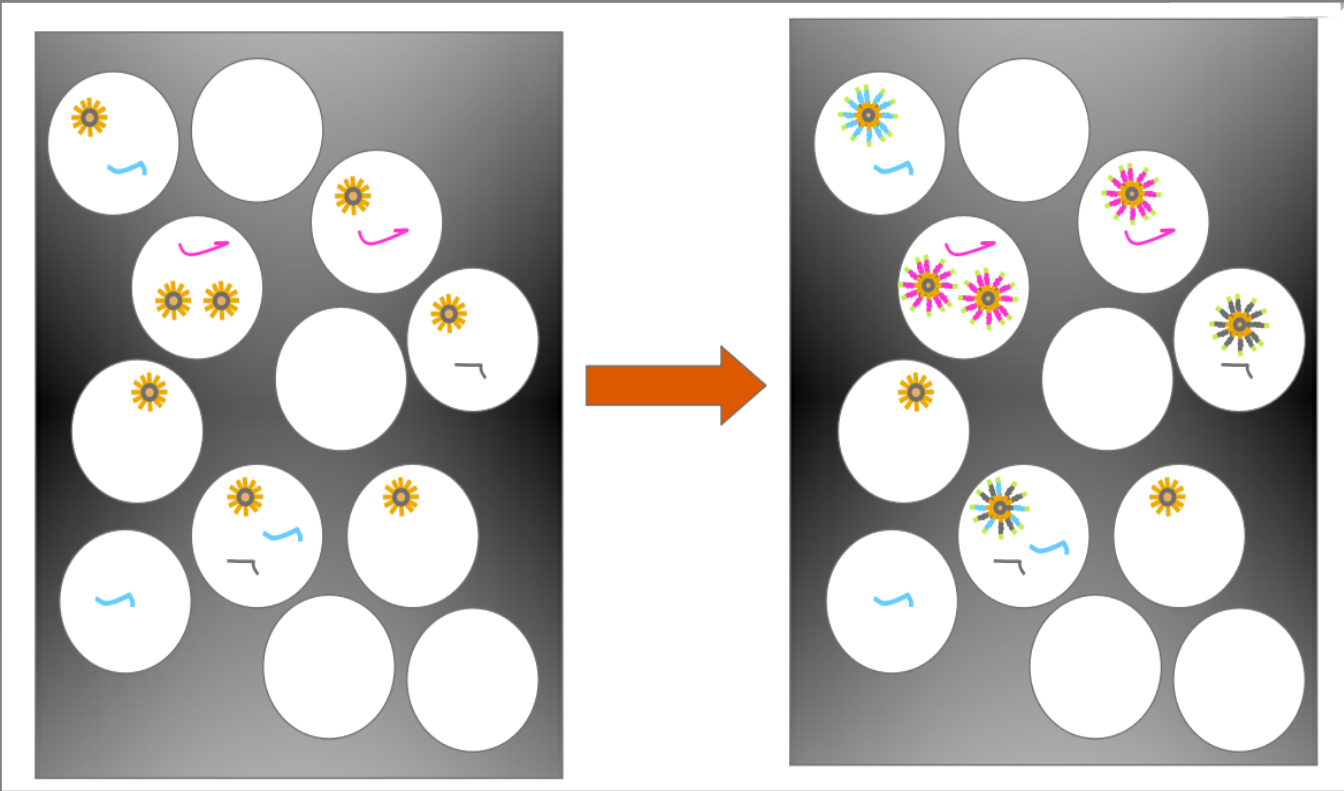
\includegraphics[scale=0.2]{epcr}
\end{figure}

\paragraph*{Why replicate DNA?}

This is a very important concept to understand, as all NGS techniques replicate DNA before sequencing is done. 

In short, DNA is replicated in order to amplify signals. No matter the method of sequencing, without a proper amount of amplification, it's near impossible to detect each base call. \\

NGS doesn't need electrophoresis, but it uses istead different methods
like the Pyrosequencing, that uses ATP and Luciferase, or Illumina
chemistry (which is the most used method today).
